% !TEX root = ../DP_Vik_Tomas_2013.tex
\chapter{Vyhodnocení}
Výsledná aplikace má model otestovaný pomocí unit testů. Ty ověřují základní funkčnost algoritmů a metod pro práci s daty modelu. Funkční a integrační testy v aplikaci přítomny nejsou.

Při vývoji aplikace byl kladen důraz na návrh uživatelského rozhranní a proto je zde kladen důraz přávě na vyhodnocení tohoto návrhu.

Důvod proč vyhodnotit návrh UI je zřejmý, výsledná aplikace má uživatelské rozhraní, které vývojář podle všech dostupných informací navrhnul tak aby bylo jednoduché na používání (viz. kapitola \ref{sec:navrh-gui}). Na konci vývojového cyklu je třeba ověřit že úsudky v návrhu byly správné.  

Během celého procesu vývoje práce byl návrh konzultován s možnými uživateli a na základě těchto konzultací a připomínek při nich získaných byl návrh upraven do finální podoby popsané v příloze \ref{chp:wireframe}.

\section{Způsoby vyhodnocení návrhu uživatelského rozhraní}
Základem vyhodnocení je uživatel a jeho práce se systémem. V této části práce budou popsány některé metody, které se používají pro zaznamenání uživatelovi činnosti, resp. pro zaznamenání okamžiků, nebo situací kdy uživatel nejednal předpokládaným způsobem. Například se v nějakém kroku od uživatele může čekat, že zadá vstup a on se místo toho pokusí odeslat formulář atp.

\subsection{Osobní konzultace}
Hlavně v ranných stádiích vývoje je nejlepší osobní kontakt s uživatelem\cite{stone2005user}. Je mnoho variací jak zvýšit efektivitu osobní konzultace.

Například je možné podporovat uživatele v tom, aby "přemýšlel nahlas" a poté si všímat, kdy se uživatelovy myšlenky odchylují od očekávaných. Tento způsob testování ovšem nění pro každého uživatele a někteří jej mohou shladat rušivým a zároveň tento způsob testování nutí uživatele více přemýšlet a provádět kroky v aplikaci momaleji (protože zároveň sděluje své myšlenky) a to může mít způsobit že uživatel neudělá chyby, které by normálně udělal.\cite{stone2005user}.

Nejvíce zpětné vazby lze získat samotným pozorováním uživatele bez toho, aby mu byla poskytnuta jakákoli pomoc při ovládání aplikace. Je možné se uživatele zeptat na otázky jako: "Co se snažíte udělat?", nebo "Co jste čekal, že se stane, když jste kliknul na to tlačítko?", ale je těžké najít správný poměr otázek tak, aby se příliš nerušila uživatelova posornost\cite{stone2005user}.

\subsection{Sezení s audiovizuálním záznamem}
Audiovizuální záznam sezení může pomoci zaznamenat přesná místa, ve kterých se uživatel dostal do problémů a zároveň slouží jako záloha pozorování, pokud by pozorovateli cokoli uniklo. Pokud se na projektu podílí více lidí, může být záznam sezení brán například jako důkaz závažnosti problému v návrhu aplikace.\cite{stone2005user}

Na obrázku \ref{fig:testing-camera} je vidět správné umístění kamery, která zabírá zároveň uživatele a zároveň obrazovku na které je zrcadlena uživatelova plocha. Tak je možné sledovat uživatele i jeho akce.\cite{stone2005user}

\begin{figure}[htb]
\begin{center}
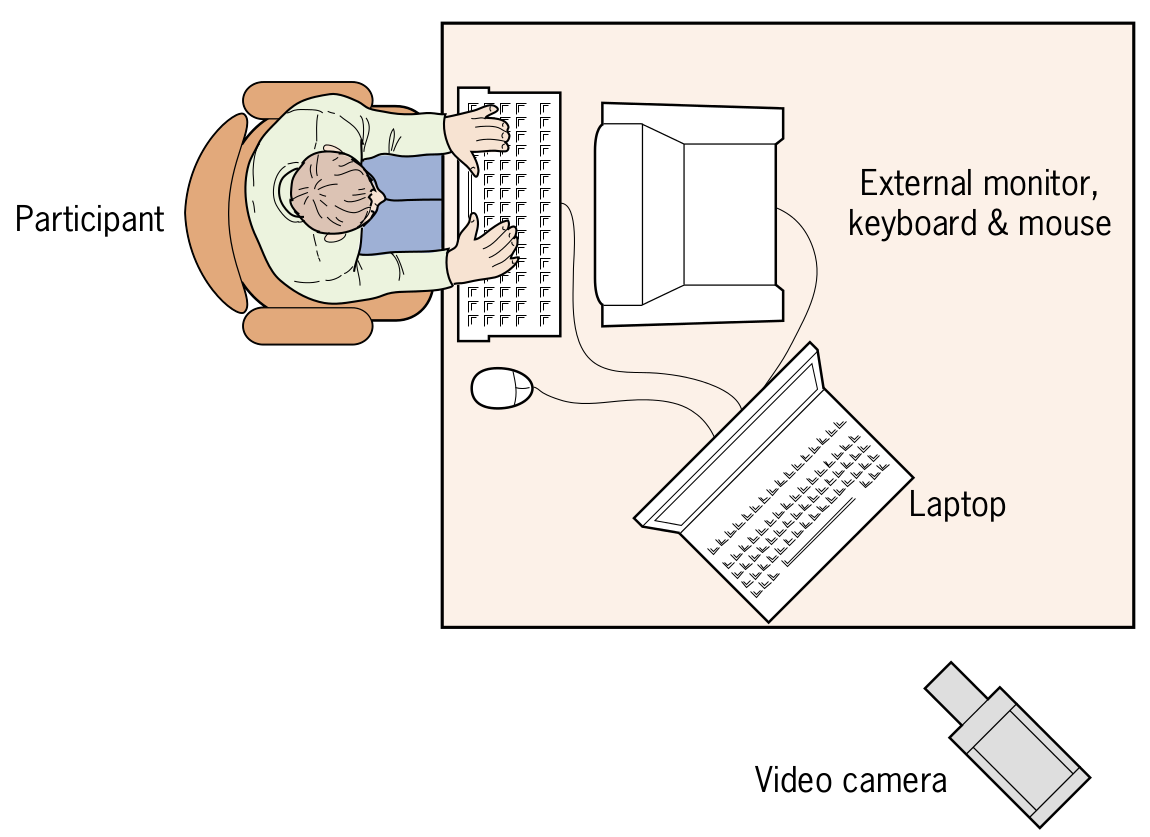
\includegraphics[width=100mm]{./pictures/testing-camera.png}
\caption{Schéma správného umístění kamery k počítačí a respondentovi\cite{stone2005user}}
\label{fig:testing-camera}
\end{center}
\end{figure}

\subsection{Sledování pohybu očí}
Metoda přesného snímání pohybu očí respondenta může odhalit chování, které nelze postřehnout ostatními metodami. Díky tomuto sledování je možné zjistit na které části obrazovky se respondent kouká a kdy se na ně kouká. Pomocí zpracování takových dat od více respondentů je možné zjistit jaká místa na obrazovce jsou jak prohlížena a tomu přizpůsobit rozmístění ovládacích prvků. Moderní zařízení pro pořízení tohoto záznamu vypadají velmi podobně jako obyčejný monitor, nebo jsou dodávana v podobě malého přídavného zařízení pod monitor (obrázek \ref{fig:tobii}).

\begin{figure}[htb]
\begin{center}
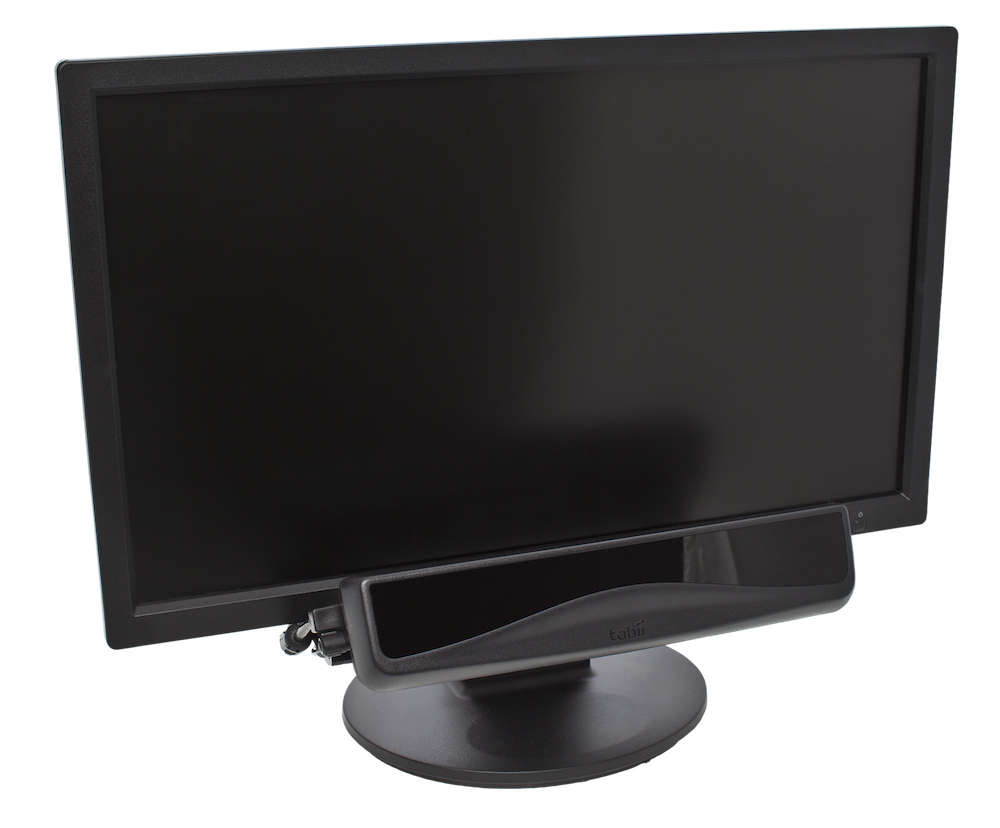
\includegraphics[width=60mm]{./pictures/tobii_image_pceye_mounted_front_rgb.jpg}
\caption{Přídavné zařízení Tobii PCEye pro sledování pohybu očí}
\label{fig:tobii}
\end{center}
\end{figure}

\subsection{Záznam akcí}
Pokud je důležité, jak rychle trvá uživateli vykonat akce v aplikaci, tedy každý klik a každý stisk klávesy se počítá, pak je vhodné použít nástroje na zaznamenávání uživatelských akcí\cite{stone2005user}. Tyto nástroje vychází ze tří základních druhů produktů\cite{stone2005user}:
\begin{itemize}
\item Produkty sledujicí že uživatel dělá svojí práci a nesnaží se narušit bezpečnost systému
\item Produkty, které nahrávají uživatelské akce za účelem pozdější prezentace této akce
\item Webové produkty které získávají informace o uživatelově pohybu mezi stránkami a četnosti návštěv.
\end{itemize}

\subsection{Dotazník}
Dotazník je jednoduchá forma získání repondentova názoru pomocí tištěné nebo elektronické verze dokumentu, ve kterém jsou otázky na témata týkající se testovaného subjektu. Otázky mohou být uzavřené, kdy uživatel může zvolit jednu z předem daných možností, nebo otevřené, kdy má uživatel možnost rozvést odpověď vlastním textem.

Použití dotazníku při vyhodnocení má mnohé výhody\cite{stone2005user}:
\begin{itemize}
\item Všechny otázky jsou napsány, na žádnou se nezapomene.
\item Všichni účastníci dostanou stejnou otázku a proto je možné mezi sebou porovnávat odpovědi.
\item Dají se pomocí něj získat kvantitativní data jako: 10 uživatelů považovalo navigaci aplikací náročnou.
\end{itemize}
Zároveň má použití dotazníku několik nevýhod\cite{stone2005user}:
\begin{itemize}
\item Je těžké dotazník navrhnout tak, aby mohl být jedinou metodou vyhodnocení. Otázky mohou zavádět, nebo nemusí mít v nabídce odpověď, která by uživateli vyhovovala.
\item Musí se předem odhadnout témata, o kterých uživatel bude chtít po testování aplikace mluvit.
\item Uzavřené otázky typu: \emph{Hodnoťe na stupnici od jedné do pěti jak jednoduchá pro vás byla navigace aplikací} jsou snadné na analyzování, ale nezjistí, proč se tak uživatel cítil.
\end{itemize}

Při tvorbě dotazníku je rozumné nejprve probrat s poteniconálním respondentem témata, které ho při práci s aplikací napadnou a ty do dotazníku zapracovat\cite{stone2005user}.

Existuje již mnoho předpřipravených dotazníků s vypracovanými metodikami vyhodnocení. Je silně doporučeno nějaký takový dotazník použít, nebo se jím minimálně nechat inspirovat\cite{stone2005user}.

\section{Popis metodiky zvolené pro tuto práci}
Pro vyhodnocení návrhu uživatelského rozhranní v této práci bude použit dotazník. Z potencionálními uživateli byl návrh konzultován průběžně a na závěrečné vyhodnocení byl zvolen dotazník pro snadnou kvantifikaci výsleků. Dotazník se skládá ze dvou částí.

První a povinnou částí je SUS dotazník. Ten vyšel nejlépe v porovnání 5ti volně dostupných dotazníků, kterou v roce 2004 prováděli Thomas S. Tullis a Jacqueline N. Stetson\cite{tullis2004comparison}. Jedná se o dotazník s deseti otázkami na které uživatel dává odpovědi v rozsahu 1-plně souhlasím až 5-vůbec nesouhlasím.

Druhou částí dotazníku jsou nepoviné otázky na funknčnost z kapitoly \ref{sec:navrh-funkcionality}. Otázky jsou zaměreny na jednotlivé funkčnosti a jejich správné a jednoduché použití uživatelem. Pro jasnou kvantifikaci byly v naprosté většině voleny uzavřené otázky.


\section{Vyhodnocení dotazníku}
